\chapter{Machine et système d'exploitation}
\section{Qu'est ce qu'un ordinateur ?}
\subsection{En théorie}
Si on tente rapidement de définir ce qu'est un ordinateur au sens large du terme (y compris tablettes, smartphones \dots), on peut lister les éléments communs suivants :
\begin{itemize}
\item un ordinateur reçoit des informations par l'intermédiaire d'un utilisateur ou d'un réseau ;
\item un ordinateur émet des informations via le réseau ou un de ses périphériques ;
\item un ordinateur a besoin d'une source d'énergie pour fonctionner.
\end{itemize}
Néanmoins cette première tentative s'avère infructueuse, on peut penser à plusieurs contre-exemples qui satisfont ces trois critères et qui ne sont pas pour autant des ordinateurs :
\begin{itemize}
\item un scooter nécessite une source d'énergie, il reçoit des informations de la part de son conducteur, il en émet sous la forme de signaux lumineux indiquant le niveau d'huile, de carburant ;
\item un interrupteur fonctionnant avec la luminosité ambiante reçoit de l'information par le biais de son capteur et transmet de l'information (ouvert-fermé), de plus le capteur nécessite une source d'énergie pour fonctionner.
\end{itemize}
Tout cela montre que la définition de ce qu'est un ordinateur n'est pas une chose si triviale que cela.\par
Pour répondre à cette question, nous allons nous aider des travaux de \textsc{Turing}. Une des grandes problématiques du siècle dernier va nous permettre de répondre à cette question : qu'est ce qu'un calcul ?\par
Dans les années trente, quatre mathématiciens au moins cherchent à répondre à cette question \textsc{Kleene}, \textsc{Church}, \textsc{Turing} et \textsc{Post}. Les question posées commencent à recevoir une réponse et c'est la naissance de la calculabilité, qui vise à définir précisément ce qui est effectivement calculable.\par 
\begin{wrapfigure}{r}{0.4\textwidth}
  \centering
  \includegraphics[width = 0.325\textwidth]{turing}
  \caption{\footnotesize{\textsc{Alan Turing}}}
\end{wrapfigure}
\textsc{Alan Turing} explore une autre approche originale, qui va lier la notion de \og calcul \fg à la notion de \og machine\fg. Il imagine une machine qui peut fonctionner sans intervention humaine. Cette machine possède les caractéristiques suivantes :
\begin{description}
\item[un ruban :] aussi long que nécessaire\footnote{Voire infini si nécessaire.}, sur lequel la machine peut lire des données et en écrire d'autres ;
\item [un état interne :] quand la machine lit un symbole, elle réagit en fonction de l'état interne en le modifiant, en réécrivant un symbole et en déplaçant éventuellement la tête vers la droite ou la gauche du symbole courant sur le ruban.
\end{description}
La machine de \textsc{Turing} est idéalisée car le ruban est supposé toujours suffisamment long (donc potentiellement infini). \textsc{Turing} va appeler \og nombre calculable\fg tout nombre qu'une machine peut écrire sur son ruban avant de s'arrêter. De même on définit alors formellement ce qu'est un algorithme  : c'est tout simplement un état interne d'une machine de \textsc{Turing}\par
Si vous voulez voir un exemple simple de fonctionnement d'une machine de \textsc{Turing}, allez voir à cette adresse : \url{http://www.espace-turing.fr/Computer-Paper-Do-It-Yourself.html}\par
Cette machine abstraite a été depuis réalisée : \url{http://videotheque.cnrs.fr/doc=3001}.\par
Un ordinateur est donc la réalisation pratique d'une machine de Turing : c'est une machine qui sert à faire des calculs. Nos ordinateurs sont en fait un peu plus compliqués afin d'être plus efficaces. \textsc{Turing} avait compris que se déplacer de case en case sur le ruban était source d'inefficacité et qu'il fallait permettre de sauter d'une case à une autre case arbitraire grâce à une adresse (il faut numéroter les cases du ruban). Actuellement on ne parle plus de ruban mais de mémoire\footnote{Qui est finie contrairement au ruban.}, cela ne change rien mais permet juste d'aller plus vite.
\subsection{Le modèle de \textsc{Von neumann}}
\subsubsection{Historique et présentation}
La première réalisation d'une machine de \bsc{turing} électronique date de 1943 pour la réalisation de l'ENIAC\footnote{Electronic Numerical Integrator Analyser and Computer}. Ce n'est pas le premier ordinateur fabriqué, il y a d'abord eu le Z3 allemand qui était mécanique.\par
\begin{wrapfigure}{r}{0.4\textwidth}
  \centering
  \includegraphics[width = 0.325\textwidth]{eckert-mauchly}
  \caption{\footnotesize{À gauche, John W. Mauchly (1907-1980) et à droite, J. Presper Eckert (1919-1995)}}
\end{wrapfigure}
\par L'ensemble fut conçu par \textsc{John William Mauchly} et \textsc{John Eckert}  et ne fut pleinement opérationnel qu'en 1946. \bsc{Von neumann} intégra l'équipe en 1944 et publia un rapport sur la conception de l'EDVAC\footnote{Electronic Discrete Variable Automatic Computer} en 1945.\par
Ce rapport d'écrit un schéma d'architecture de calculateur, organisé en trois éléments (unité arithmétique, unité de commande et mémoire contenant programme et données). Il décrit aussi des principes de réalisation pour ces éléments, notamment les opérations arithmétiques. Si ce dernier aspect dépend partiellement de la technologie connue à l'époque, et a donc nécessairement vieilli, le modèle d'architecture, qui marque une transition profonde avec les pratiques antérieures, reste d'une étonnante actualité. Ce modèle, auquel reste attaché le nom de von Neumann, est représenté par le schéma de la figure \ref{fig:neumann}.
\begin{figure}[ht]
  \centering
  \begin{tikzpicture}[> = triangle 45]
    \node at (-1cm,0) [fill = blue!20,draw, rounded corners, minimum height = 5cm,minimum width = 4cm] (mem) (mem) {\Large{Mémoire}};
    \node at (5cm,1.5cm) [fill = blue!20,draw, rounded corners, minimum height = 2cm ,minimum width = 4cm, text width = 2cm] (com) {Unité de commande};
    \node at (5cm,-1.25cm) [fill = blue!20,draw, rounded corners, minimum height = 2.5cm,minimum width = 4cm, text width = 3cm] (arit) {Unité arithmétique et logique};
    \node at (5,-2.1) [fill = yellow!20,draw, shape = rectangle, minimum width = 3.5cm] (accu) {accumulateur};
    \node at (5,0) [orange, draw, rounded corners, minimum height = 5.5cm ,minimum width = 4.5cm, line width = 1.2mm] (proc) {};
    \draw[orange, line width = 1mm] (proc.east)++(0.2,1.5) -- ++(1,0) node[black,anchor = west, text width = 3cm] {Unité centrale ou processeur};
    \node at (10,-1.5) [fill = pink!50, shape = rectangle, minimum width = 3 cm] (ent) {Entrées};
    \node at (10,-2.6) [fill = pink!50, shape = rectangle, minimum width = 3 cm] (sort) {Sorties};
    \draw[->, line width = 0.8mm, red] (com.west)++(0,0.5) -- ++(-2.00cm,0) node[midway, above] {Bus};
    \draw[<-, line width = 0.8mm, red] (com.west)++(0,-0.5) -- ++(-2.00cm,0);
    \draw[->, line width = 0.8mm, red] (arit.west)++(0,0.5) -- ++(-2.00cm,0);
    \draw[<-, line width = 0.8mm, red] (arit.west)++(0,-0.5) -- ++(-2.00cm,0);
    \draw[->, line width = 0.8mm, red] (arit.north)++(-0.5,-0.5) -- ++(0,1.5);
    \draw[<-, line width = 0.8mm, red] (arit.north)++(0.5,-0.5) -- ++(0,1.5) node[midway, right] {Bus};
    \draw[<-, line width = 0.8mm, red] (accu.east)++(0,0.1) -- (ent.west) node[pos = 0.6,sloped,above] {Bus};
    \draw[->, line width = 0.8mm, red] (accu.east)++(0,-0.1) -- (sort.west);
  \end{tikzpicture}
  \caption{\label{fig:neumann}\footnotesize{Le modèle originel de von Neumann pour l'architecture des ordinateurs.}}
 \end{figure}
Il y a schématiquement quatre composants principaux :
\begin{description}
\item[le processeur :] qui se décompose en une unité de commande et une unité arithmétique et logique ;
\item[la mémoire :] qui contient des instructions et des données ;
\item[les périphériques d'entrée-sortie :] qui permettent une communication entre l'utilisateur et les machine (via clavier, souris, écran \dots) ;
\item[le bus :] qui est le canal de communication entre la mémoire, le processeur et les périphériques.
\end{description}
\par La première innovation est la séparation nette entre l'unité de commande, qui est chargée d'organiser le flot des instructions, et l'unité arithmétique, chargée de l'exécution proprement dite de ces instructions\footnote{En gros les calculs.}. La seconde innovation est l'idée du programme enregistré, fini les rubans, cartes à trous \dots Les instructions et les données sont maintenant enregistrées dans la mémoire selon un codage conventionnel. Un compteur ordinal ou pointeur d'instruction, contient l'adresse de l'instruction en cours d'exécution ; il est automatiquement incrémenté après exécution de l'instruction, et explicitement modifié par les instructions de branchement comme le \lstinline?if?, le \lstinline?while? ou le vénérable \lstinline?goto? du basic\footnote{Qu'on retrouve toujours en assembleur.}.
\subsubsection{Le rôle de chaque élément}
\paragraph{Le processeur.}
Le processeur est le cerveau de l'ordinateur, il donne des ordres aux périphériques et à la mémoire et est responsable de l'exécution du programme de l'ordinateur.\par
Le processeur dispose d'une toute petite mémoire, typiquement de l'ordre de quelques mots à une centaine de mots, qu'on appelle des registres. La fonction du registre de données (mémoire rapide) est de contenir les données transitant entre l'unité de traitement et l'extérieur.\par
 La fonction de l'accumulateur est principalement de contenir les opérandes ou les résultats des opérations de l'unité arithmétique et logique.\par
Son unité arithmétique et logique permet de réaliser les calculs :
\begin{itemize}
\item opérations arithmétiques binaires: addition, multiplication, soustraction, division ;
\item opérations logiques, conjonction, disjonction et négation.
\end{itemize}
L'unité de contrôle accède à la mémoire via le bus, possibilité de lecture d'une case mémoire et d'écriture dans une case mémoire. Cependant cette unité ne contient pas le programme à exécuter : les instructions à exécuter sont codées sous la forme d'une suite de bits stockée en mémoire. Toutes les instructions sont réalisées dans l'ordre sauf le cas particulier des instructions de branchement ou de saut :
\begin{itemize}
\item une instruction conditionnelle indique la prochaine instruction à réaliser en fonction du résultat d'un calcul logique ;
\item une instruction répétitive doit être réalisée plusieurs fois.
\end{itemize}
\paragraph{La mémoire.}
La mémoire est une suite de chiffes binaires nommés \emph{bits}, organisés en paquets de huit (les \emph{octets}) puis en mots mémoire de 64 bits\footnote{Sur le machines anciennes c'est plutôt 32 bits.}. Un mot en mémoire peut représenter plusieurs choses : une instruction, un entier \dots La signification du mot dépend de l'utilisation qu'on en fait.\par
La mémoire ne sert qu'à stocker ces mots, elle ne réalise aucune opération et n'effectue aucun calcul. Chaque mot possède une adresse, avec cette adresse on peut lire un mot ou alors écrire un autre mot à la place. Cette adresse est attribuée de manière aléatoire\footnote{Contrairement aux disques durs par exemple où les lecture et écritures se font dans un ordre déterminé.} d'où le nom de \emph{Random access memory} (\emph{RAM}). 
\paragraph{Les périphériques.} De manière formelle il s'agit de mémoire supplémentaire dans laquelle le processeur peut écrire pour donner des ordres au périphérique (afficher telle couleur sur tel pixel de l'écran) ou lire (réagir à telle touche tapée sur un clavier).
\subsubsection{Avantages et inconvénients}
L'architecture de \textsc{Von Neumann} permet une grande souplesse car on peut stocker virtuellement n'importe quels types de structures en mémoire notamment des données ou des programmes.\par
Par contre cet architecture possède trois inconvénients :
\begin{description}
\item[monotâche :] les instructions sont exécutées de manière séquentielle, les unes après les autres, une machine de \textsc{Von Neumann} ne permet donc de ne faire qu'une seule chose à la fois\footnote{Nous verrons plus loin comment les systèmes d'exploitation permettent de s'affranchir de cette limitation.} ;
\item[le bus :] durant ces dernières années, de gros efforts se sont portés sur l'amélioration de la vitesse de calcul des processeurs ; ils sont actuellement si rapides que le processeur passe beaucoup de temps à attendre que les données précédentes soit transférées avant d'en envoyer de nouvelles ;
\item[faible robustesse :] les données et les programmes étant stockés dans la même mémoire, si un bogue d'un programme provoque une écriture à un endroit non désiré, cela peut compromettre le fonctionnement de l'ensemble de la machine.
\end{description}
\subsubsection{De nos jours}
L'architecture de \textsc{Von neumann} a peu évoluée de puis sa création. Néanmoins il existe quelques petites différences :
\begin{description}
\item[mémoire morte : ] la RAM nécessite un apport constant d'énergie pour fonctionner, une simple coupure de courant peut mettre en péril tous les calculs et programmes réalisés ; on sait de nos jours construire des mémoires non volatiles permettant un accès en lecture mais pas en écriture (\emph{Read Only Memory} : ROM) ; elles sont utilisés de nos jours pour stocker un programme particulier servant au démarrage de la machine (firmware ou BIOS) ; cette mémoire ne permet pas de stocker les données utilisateurs ;
\item[mémoire de masse :] pour stocker ces données utilisateurs on utilise de nos jours des disques durs (souvent pour les ordinateurs\footnote{L'augmentation des la taille de ces disques durs est liée à la découverte de la magnéto-résistance géante qui a valu le prix \textsc{Nobel} à ses découvreurs \textsc{Albert Fert} et \textsc{Peter Grünberg}.}) ou une mémoire flash (souvent pour les smartphones) ;
\end{description}
De plus certains périphériques peuvent accéder directement à la mémoire sans passer par le processeur, on pare alors de \emph{Direct Memory Access} ou DMA, et certains calculs d'affichage sont laissés à un processeur spécialisé possédant une mémoire vive importante présent sur la carte graphique.\par
Les ordinateurs comportent maintenant des processeurs multiples, qu'il s'agisse d'unités séparées ou de \og cœurs \fg multiples à l'intérieur d'une même puce. Cela permet d'obtenir une puissance de calcul plus élevée sans augmenter la puissance d'un processeur individuel qui est limitée par les capacités d'évacuation de la chaleur\footnote{Effet \textsc{Joule}, quand tu nous tiens.} dans des circuits de plus en plus denses. Ainsi l'architecture actuelle ressemble plus à celle que vous pouvez voir sur la figure \ref{fig:newneumann}.
\begin{figure}[ht]
  \centering
  \begin{tikzpicture}[> = triangle 45]
    \node at (1,3) [fill = pink!50, shape = rectangle, minimum width = 3 cm] (ent) {Entrées};
    \node at (1,1) [fill = pink!50, shape = rectangle, minimum width = 3 cm] (sort) {Sorties};
     \node at (6,2) [fill = blue!20,draw, rounded corners, minimum height = 5cm,minimum width = 4cm] (mem) (mem) {\Large{Mémoire}};
     \node at (10,4) [fill = blue!20,draw, rounded corners, minimum width = 1.5 cm] (uc1) {UC};
     \node at (10,3.2) [fill = blue!20,draw, rounded corners, minimum width = 1.5 cm] (ual1) {UAL};
     \node at (10,3.6) [orange, draw, rounded corners, minimum height = 1.8cm, minimum width = 2cm, line width = 1mm] (proc1) {};
     \node at (10,.8) [fill = blue!20,draw, rounded corners, minimum width = 1.5 cm] (uc2) {UC};
     \node at (10,0) [fill = blue!20,draw, rounded corners, minimum width = 1.5 cm] (ual2) {UAL};
     \node at (10,0.4) [orange, draw, rounded corners, minimum height = 1.8cm, minimum width = 2cm, line width = 1mm] (proc2) {};
     \draw[->, red] (uc1.south) ++(-0.5,0.2) -- ++(0,-0.5);
     \draw[<-, red] (uc1.south) ++(0.5,0.2) -- ++(0,-0.5);
     \draw[->, red] (uc2.south) ++(-0.5,0.2) -- ++(0,-0.5);
     \draw[<-, red] (uc2.south) ++(0.5,0.2) -- ++(0,-0.5);
     \draw[->, red, line width = 0.6mm] (ent.east) -- ++(1.5,0);
     \draw[<-, red, line width = 0.6mm] (sort.east) -- ++(1.5,0);
     \draw[->, red, line width = 0.6mm] (mem.east)++(0,1.4) -- ++(1,0);
     \draw[<-, red, line width = 0.6mm] (mem.east)++(0,2) -- ++(1,0); 
     \draw[->, red, line width = 0.6mm] (mem.east)++(0,-1.4) -- ++(1,0);
     \draw[<-, red, line width = 0.6mm] (mem.east)++(0,-2) -- ++(1,0); 
     \node at (10,2) [red] {\Huge{\dots}};
     \node at (12,2) [blue!80, rotate around={-90:(0,0)}] {\Large{Processeurs}};
  \end{tikzpicture}
  
  \caption{\label{fig:newneumann}\footnotesize{Le modèle de \textsc{Von Neumann} aujourd'hui}}

\end{figure}
\section{En pratique}
Dans cette partie nous allons voir comment on réalise en pratique des éléments capables de réaliser des calculs et de stocker des objets en mémoire. Nous allons considérer que l'élément fondamental est le transistor et nous allons expliquer son fonctionnement sans pour autant décrire précisément sa structure et sa fabrication : nous n'allons donc pas expliquer la jonction PN et le dopage des semi-conducteurs\footnote{Pour ceux que ça intéresse, vous pouvez aller visiter visiter ce site : \url{http://fr.wikipedia.org/wiki/Dopage_(semi-conducteur)}.}. On pourrait aller encore plus loin en considérant les calculs réalisés par ordinateur sont le résultat de mouvements d'électrons dans un champ électrique très complexe.
\subsection{L'élément fondamental : le transistor}
Le transistor est la brique avec laquelle sont construits les micro-processeurs, la RAM et la ROM. La technologie actuellement utilisée pour fabriquer les micro-processeurs est la technologie MOS (Metal-Oxide-Semiconductor). Il existe deux types de transistors MOS : les transistors de type n et les transistors de type p. Les micro-processeurs actuels utilisent des transistors des deux types. On parle alors de technologie CMOS (Complementary Metal-Oxide-Semiconductor).
\par Un transistor est un composant électronique qui possède trois pôles par lesquels il est relié au reste du circuit. Ces trois pôles sont appelés drain, grille et source pour les transistors MOS ou alors collecteur, base et émetteur pour les transistors bipolaires.
\par Dans le cas des transistors MOS, le drain et la source jouent des rôles (presque) symétriques et sont (pratiquement) interchangeables. Un transistor se comporte comme un interrupteur électrique entre la source et le drain qui serait commandé par la grille. Le symbole électrique d'un transistor est donné sur la figure \ref{fig:trans}.
\begin{figure}[ht]
  \centering
  \begin{circuitikz}
  \draw (0,0) node[nmos] (mos) {} 
  (mos.gate) node[anchor=east] {Grille}
  (mos.drain) node[anchor=south] {Drain}
  (mos.source) node[anchor=north] {Source};

  \draw (4,0) node[pmos] (pmos) {} 
  (pmos.gate) node[anchor=east] {Grille}
  (pmos.drain) node[anchor=north] {Drain}
  (pmos.source) node[anchor=south] {Source};
  \end{circuitikz}
  \caption{\footnotesize{Transistor n-MOS et p-MOS}}
  \label{fig:trans}
\end{figure}
\par En première approximation, le comportement d'un transistor n-MOS est le suivant :
\begin{itemize}
\item si la tension entre la grille et la source $V_{GS}$ est supérieure à une tension de seuil\footnote{$th$ pour threshold qui signifie seuil en anglais.} $V_{th}$, la source et le drain sont connectés ;
\item si au contraire, la tension entre la grille et la source $V_{GS}$ est mise inférieure à cette tension de seuil, le circuit entre la source et le drain est ouvert.
\end{itemize}
Ainsi un transistor n'est rien qu'un interrupteur qui est commandé par la tension qu'on applique entre la grille et la source. La tension de seuil est caractéristique du transistor mais dépend aussi de facteurs extérieurs, en particulier la température, mais elle est en général comprise entre 0,8 V et 4 V. Les schémas équivalents sont donnés sur la figure \ref{fig:trans2}.
\begin{figure}[ht]
  \centering
  \begin{tikzpicture}
  \draw (0,0) node[nmos] (mos) {};
  \draw (mos.gate) to [R=$R$] ++(-2,0) to [V, v_<=$e$] ++(0, -2) -| (mos.source);
  \draw (mos.drain) -- ++(1,0) to [R=Circuit] ++(0,-2) -| (mos.source);
  \draw (3,-1) node {$\Leftrightarrow$};
  \begin{scope}[xshift=5cm]
    \draw (0,0) to [V=$e > V_{th}$] (0,2) to [R=$R$] (2,2) -- ++(0,-2) -| (0,0);
    \draw (2,2) -- ++(0,1) -- ++(1,0) to [R=Circuit] ++(0,-2) -- ++(-1,0);
  \end{scope}
  \begin{scope}[xshift=5cm,yshift=-4cm]
    \draw (0,0) to [V=$e < V_{th}$] (0,2) to [R=$R$] (2,2) to[ospst] ++(0,-1) -- ++(0,-1) -| (0,0);
    \draw (2,2) to [ospst] ++(0,1) -- ++(1,0) to [R=Circuit] ++(0,-2) -- ++(-1,0);
  \end{scope}
  \end{tikzpicture}
  \caption{\footnotesize{Circuits équivalents d'un transistor n-MOS en fonctionnement}}
  \label{fig:trans2}
\end{figure}
\par Le fonctionnement d'un transistor p-MOS est l'inverse. Le drain et la source sont connectés lorsque la tension appliquée entre la grille et la source est inférieure à $-V_{th}$.
\subsection{Réalisation de portes logiques}
Vous avez vu dans le chapitre \ref{chap:bool} que les connecteurs logiques permettent de faire des opérations simples. En fait on peut réaliser avec des circuits logiques des opérations sur les nombres binaires comme l'addition, la multiplication \dots Il est donc important de savoir réaliser un composant électronique permettant de simuler un connecteur logique afin de pouvoir faire ces opérations avec un processeur.
\subsubsection{Conventions}
En logique on travaille avec les booléens, on considèrera comme un 1 ou \lstinline?True? toute tension supérieure à la tension de seuil $V_{th}$ et comme un 0 ou \lstinline?False? toute tension inférieure à $V_{th}$. Dans le cadre des conventions actuelles on choisit une tension de 5 V pour le 1 ou \lstinline?True? et de 0 V pour le 0 ou \lstinline?False?\par
De plus comme il risque d'y avoir beaucoup de composants et de fil, pour simplifier la réalisation des schémas on considère que lorsque deux fils se croisent il n'y a pas de connexion des deux fils sauf si l'intersection est matérialisé par un point comme sur la figure \ref{fig:conn}.
\begin{figure}[ht]
  \centering
  \begin{circuitikz}
    \draw (0,0) -- (2,0);
    \draw (1,-1) -- (1,1) node[anchor = south] {Pas de connexion} ;
    \begin{scope}[xshift=4cm]
\draw (0,0) -- (2,0);
    \draw (1,-1) to [short,-*] (1,0) -- (1,1) node[anchor = south] {Connexion} ;      
    \end{scope}
  \end{circuitikz}
  \caption{\footnotesize{Convention des connexions aux intersections}}
  \label{fig:conn}
\end{figure}
\subsubsection{La porte Non}
C'est la porte la plus simple à réaliser. On rappelle la table de vérité de cet opérateur :
\begin{center}
  \begin{tabular}{|c|c|}
    \hline
    Entrée & Sortie\\
    $p$ & $\overline p$ ou $\lnot p$\\
    \hline
    1 & 0\\
    0 & 1\\
    \hline
  \end{tabular}
\end{center}
Son schéma est donné sur la figure \ref{fig:not}.
\begin{figure}[ht]
  \centering
  \begin{circuitikz}
    \draw (2,1) node[pmos] (pmos) {};
    \draw (2,-1) node[nmos] (nmos) {};
    \draw (pmos.gate) -- ++(-1,0) |- (nmos.gate);
    \draw (-1,0) node[anchor = east] {$p$} to [short,-*] ++(1,0);
    \draw (pmos.source) -- ++(0,0.5) node[anchor = south] {1} -- ++(0.5,0) -- ++(-1,0);
    \draw (nmos.source) -- ++(0,-0.5) node[anchor = north] {0} -- ++(0.5,0) -- ++(-1,0);
    \draw (pmos.drain) -- (nmos.drain);
    \draw (pmos.drain) ++(0,-0.25) to [short,*-] ++(1,0) node[anchor=west] {$\overline p$};
    \draw (6.5,1) node[european not port] (not) {};
    \draw (not.in) node[anchor=east] {$p$};
    \draw (not.out) node[anchor = west] {$\overline p$};
    \draw (6,-1) node[american not port] (anot) {};
    \draw (anot.in) node[anchor=east] {$p$};
    \draw (anot.out) node[anchor = west] {$\overline p$};
  \end{circuitikz}
  \caption{\footnotesize{La porte Non et son symbole européen en haut et américain en bas}}
  \label{fig:not}
\end{figure}
\subsection{Porte Non Et et Non Ou}
la porte Non Et et la porte Non Ou sont en pratique plus simples à réaliser que les portes Et et Ou. Cela provient du fait que la source et le drain des transistors ne jouent pas des rôles complètement symétriques. Pour des raisons de consommation, les connexions avec le 0 sont toujours commandées par des transistors de type n et les connexions avec le 1 par des transistors de type p.\par 
On donne dans le tableau suivant les tables de vérités de ces deux opérateurs :
\begin{center}
  \begin{tabular}{|c|c|c|c|}
    \hline
    $p$ & $q$ & $\overline{p \land q}$ & $\overline{p \lor q}$\\
    \hline
    0 & 0 & 1 & 1 \\
    0 & 1 & 1 & 0 \\
    1 & 0 & 1 & 0 \\
    1 & 1 & 0 & 0\\
    \hline
  \end{tabular}
\end{center}
On donne sur la figure \ref{fig:nonet} la réalisation de la porte Non Et avec quatre transistors. De même sur la figure \ref{fig:nonou} vous avez la réalisation de la porte Non Ou avec quatre transistors.
\begin{figure}[ht]
  \centering
  \begin{circuitikz}
    \draw (0,2) node[pmos] (pmos1) {};
    \draw (2,2) node[pmos] (pmos2) {};
    \draw (2,0) node[nmos] (nmos1) {};
    \draw (2,-2) node[nmos] (nmos2) {};
    \draw (pmos1.source) -- ++(0,0.5) ++(-1,0) -- ++(4,0) node[anchor=west] {1};
    \draw (pmos2.source) -- ++(0,0.5);
    \draw (pmos2.drain) -- (nmos1.drain);
    \draw (nmos1.source)-- (nmos2.drain);
    \draw (nmos2.source) -- ++(0,-0.5) ++(-0.5,0) -- ++(1,0) node[anchor=west] {0};
    \draw (pmos2.gate) -- ++(-0.5,0) |- (nmos2.gate);
    \draw (nmos2.gate) ++(-0.5,0) -- ++(-3,0) node[anchor=east] {$q$};
    \draw (nmos1.gate) -- ++(-3.5,0) node[anchor=east] {$p$};
    \draw (pmos1.gate) -- ++(-0.5,0) -- ++(0,-2);
    \draw (pmos1.drain) -- ++(0,-0.25) to [short,-*] ++(2,0) -- ++(0.5,0) node[anchor=west] {$\overline{p \land q}$};
    \begin{scope}[xshift=7cm]
      \draw (0,2) node[european nand port] (nand) {};
      \draw (nand.in 1) node[anchor = east] {$p$};
      \draw (nand.in 2) node[anchor = east] {$q$};
      \draw (nand.out) node[anchor = west] {$\overline{p \land q}$};
      \draw (0,-2) node[american nand port] (nand) {};
      \draw (nand.in 1) node[anchor = east] {$p$};
      \draw (nand.in 2) node[anchor = east] {$q$};
      \draw (nand.out) node[anchor = west] {$\overline{p \land q}$};
    \end{scope}
  \end{circuitikz}
  \caption{\footnotesize{La porte Non Et et son symbole européen en haut et américain en bas}}
  \label{fig:nonet}
\end{figure}
\begin{figure}[h!]
  \centering
\begin{circuitikz}
\draw (2,2) node[pmos] (pmos1) {};
\draw (2,0) node[pmos] (pmos2) {};
\draw (2,-2) node[nmos] (nmos1) {};
\draw (0,-2) node[nmos] (nmos2) {};
\draw (pmos1.gate) -- ++(-0.5,0) |- (nmos1.gate);
\draw (pmos1.source) -- ++(0,0.5) ++(-0.5,0) -- ++(1,0) node[anchor=west] {1};
\draw (nmos2.source) -- ++(0,-0.5) ++(-0.5,0) -- ++(3,0) node[anchor=west] {0};
\draw (nmos1.source) -- ++(0,-0.5);
\draw (pmos2.gate) -- ++(-2.5,0) |- (nmos2.gate);
\draw (pmos2.gate) ++(-2.5,0) -- ++(-0.5,0) node[anchor=east] {$q$};
\draw (nmos2.drain) -- ++(0,0.25) to [short,-*] ++(2,0) -- ++(0.5,0) node[anchor=west] {$\overline{p\lor q}$}; 
\draw (pmos2.drain) -- (nmos1.drain);
\draw (pmos1.drain) -- (pmos2.source);
\draw (pmos1.gate) ++(-0.5,0) -- ++(-2.5,0) node[anchor=east] {$p$};
\begin{scope}[xshift=7cm]
      \draw (0,2) node[european nor port] (nor) {};
      \draw (nor.in 1) node[anchor = east] {$p$};
      \draw (nor.in 2) node[anchor = east] {$q$};
      \draw (nor.out) node[anchor = west] {$\overline{p \lor q}$};
      \draw (0,-2) node[american nor port] (nor) {};
      \draw (nor.in 1) node[anchor = east] {$p$};
      \draw (nor.in 2) node[anchor = east] {$q$};
      \draw (nor.out) node[anchor = west] {$\overline{p \lor q}$};
    \end{scope}
\end{circuitikz}
\caption{\footnotesize{La porte Non Ou et son symbole européen en haut et américain en bas}}
  \label{fig:nonou}
\end{figure}
\subsection{Porte Et, porte Ou}
La réalisation de ces deux portes est maintenant toute simple, il suffit d'associer une porte Non Et avec une porte Non pour avoir une porte Et. Pour la porte Ou, il suffit d'associer une porte Non Ou avec une porte Ou. Tout cela est schématisé sur la figure \ref{fig:Etou}.
\begin{figure}[ht]
  \centering
  \begin{circuitikz}
    \draw (0,0) node[european nand port] (nand) {};
    \draw (nand.in 1) node[anchor=east] {$p$};
    \draw (nand.in 2) node[anchor=east] {$q$};
    \draw (2,0) node[european not port] (not1) {};
    \draw (nand.out) -- (not1.in);
    \draw (not1.out) node[anchor=west] {$p\land q$};
    \draw (6,0) node[european nor port] (nor) {};
    \draw (nor.in 1) node[anchor=east] {$p$};
    \draw (nor.in 2) node[anchor=east] {$q$};
    \draw (8,0) node[european not port] (not2) {};
    \draw (nor.out) -- (not2.in);
    \draw (not2.out) node[anchor=west] {$p\lor q$};
  \end{circuitikz}
  \caption{\footnotesize{Porte Et, porte Ou}}
  \label{fig:Etou}
\end{figure}
\subsection{Mémoire}
On appelle mémoire un composant électronique permettant de stocker une information sous forme binaire. Les mémoires des tous premiers ordinateurs étaient magnétiques. Les mémoires sont maintenant des composants électroniques à base de transistors. Il existe deux types de mémoires qui se distinguent par leur technique de fabrication : les mémoires dynamiques et les mémoires statiques. Il s'agit dans les deux cas de mémoires volatiles qui nécessitent une alimentation pour conserver leur contenu. La mémoire dynamique est appelée DRAM pour Dymanic RAM par opposition à la mémoire statique appelée SRAM pour Static RAM.\par
La mémoire dynamique est utilisée pour la mémoire principale de l'ordinateur car son coût est moindre et sa miniaturisation plus aisée. Par contre, la mémoire statique est utilisée pour les caches en raison de sa plus grande vitesse.
\subsubsection{Mémoire dynamique}
Chaque élément de mémoire dynamique est formé d'un condensateur et d'un transistor de commande agencés comme indiqué sur la figure \ref{fig:dynmem}. 
\begin{figure}[ht]
  \centering
  \begin{circuitikz}
    \draw (0,0) node[nmos, rotate around={-90:(0,0)}] (nmos) {};
    \draw (nmos.gate) -- ++(0,0.5) ++(-0.5,0) -- ++(1,0) node[anchor=west] {$A$};
    \draw (nmos.source) -- ++(-1,0) ++(0,0.5) -- ++(0,-1) node[anchor = north] {$B$};
    \draw (nmos.drain) -- ++(0.5,0) to [C= $C$] ++(0,-1) to node[ground] {} ++(0,-0.1);
  \end{circuitikz}
  \caption{\footnotesize{Mémoire dynamique 1 bit}}
  \label{fig:dynmem}
\end{figure}
La ligne $A$ est appelée ligne de commande ou ligne d'adresse. La ligne $B$ est la ligne de donnée sur laquelle est lu ou écrit le bit d'information. Le bit d'information est représenté par la tension aux bornes du condensateur. Lorsque la ligne de commande est à 0, le condensateur est isolé et la charge du condensateur reste constante\footnote{En première approximation seulement car un condensateur possède une résistance de fuite au travers de laquelle il se décharge lentement.} tout comme la tension à ses bornes. Au contraire, lorsque la ligne de commande est à 1, on peut lire soit le bit en mesurant la tension aux bornes du condensateur, soit écrire un nouveau bit en appliquant la tension voulue aux bornes du condensateur.
\subsubsection{Mémoire statique}
Chaque élément de mémoire statique est formé de six transistors. Quatre de ces six transistors constituent deux porte Non mises tête-bêche et les deux derniers, commandés par la ligne d'adresse A, relient les inverseurs aux lignes de données comme sur la figure \ref{fig:memstat}.
\begin{figure}[ht]
  \centering
  \begin{circuitikz}
    \draw (0,3) node[nmos] (nmos1) {};
    \draw (0,1) node[european not port] (not1) {};
    \draw (0,-1) node[european not port] (not2) {};
    \draw (0,-3) node[nmos] (nmos2) {};
    \draw (not1.out) -- ++(0.5,0) -- ++(0,-0.5) -- ++(-3,-1) |- (not2.in);
    \draw (not2.out) -- ++(0.5,0) -- ++(0,0.5) -- ++(-3,1) |- (not1.in);
    \draw (nmos1.gate) -- ++(-2,0) |- (nmos2.gate);
    \draw (nmos1.gate) ++(-2,0) -- ++(-0.5,0) node[anchor=east] {$A$};
    \draw (not1.out) ++(0.5,0) |- (nmos1.source);
    \draw (not2.out) ++(0.5,0) |- (nmos2.drain);
    \draw (nmos1.drain) -- ++(0.5,0) node[anchor=west] {$B$};
   \draw (nmos2.source) -- ++(0.5,0) node[anchor=west] {$\overline B$}; 
  \end{circuitikz}
  \caption{\footnotesize{Mémoire statique 1 bit}}
  \label{fig:memstat}
\end{figure}
Comme pour la mémoire dynamique, il est nécessaire d'alimenter la ligne d'adresse si on veut faire quoi que ce soit. Une fois la ligne d'adresse alimentée, on peut mesurer la tension de sortie des portes Non ou la modifier. Pour la suite on ne représentera plus ces lignes d'adresses et on les considèrera comme alimentée pour étudier le fonctionnement de la mémoire. Ainsi cette mémoire statique sera représentée sans la ligne d'adresse et sans les deux transistors qui la relie aux portes Non (voir la figure \ref{fig:memstat2}).
\begin{figure}[ht]
  \centering
  \begin{circuitikz}
    \draw (0,1) node[european not port] (not1) {};
    \draw (0,-1) node[european not port] (not2) {};
    \draw (not1.out) -- ++(0.5,0) -- ++(0,-0.5) -- ++(-3,-1) |- (not2.in);
    \draw (not2.out) -- ++(0.5,0) -- ++(0,0.5) -- ++(-3,1) |- (not1.in);
    \draw (not1.out) ++(0.5,0) -- ++(0.5,0) node[anchor=west] {$B$};
    \draw (not2.out) ++(0.5,0) -- ++(0.5,0) node[anchor=west] {$\overline B$}; 
  \end{circuitikz}
  \caption{\footnotesize{Représentation simplifiée de la mémoire statique 1 bit}}
  \label{fig:memstat2}
\end{figure}
\par Le fonctionnement est très simple, le bit est lu sur la sortie $B$. Pour changer la valeur stockée en mémoire, il suffit de modifier la tension en sortie de la seconde porte non $\overline B$.\par
Il existe d'autres réalisations possibles de mémoire statique avec des portes Nand et Nor qu'on appelle verrou SR. L'avantage de ces mémoires est que l'écriture se fait avec deux entrées séparées, une pour le 0 (entrée R pour Reset) et une pour le 1 (entré S pour Set). Deux exemples sont donnés sur la figure \ref{fig:memstat3}.
\begin{figure}[ht]
  \centering
  \begin{circuitikz}
    \draw (0,2) node[european nor port] (nor1) {};
    \draw (0,0) node[european nor port] (nor2) {};
    \draw (nor1.out) -- ++(0.5,0) -- ++(0,-0.5) -- ++(-3,-1) |- (nor2.in 1);
    \draw (nor2.out) -- ++(0.5,0) -- ++(0,0.5) -- ++(-3,1) |- (nor1.in 2);
    \draw (nor1.in 1) -- ++(-1,0) node[anchor=east] {$R$};
    \draw (nor2.in 2) -- ++(-1,0) node[anchor=east] {$S$};
    \draw (nor1.out) ++(0.5,0) -- ++(0.5,0) node[anchor=west] {$B$};
    \draw (nor2.out) ++(0.5,0) -- ++(0.5,0) node[anchor=west] {$\overline B$};
    \begin{scope}[xshift=6cm]
      \draw (0,2) node[european nand port] (nand1) {};
      \draw (0,0) node[european nand port] (nand2) {};
      \draw (nand1.out) -- ++(0.5,0) -- ++(0,-0.5) -- ++(-3,-1) |- (nand2.in 1);
      \draw (nand2.out) -- ++(0.5,0) -- ++(0,0.5) -- ++(-3,1) |- (nand1.in 2);
      \draw (nand1.in 1) -- ++(-1,0) node[anchor=east] {$\overline S$};
      \draw (nand2.in 2) -- ++(-1,0) node[anchor=east] {$\overline R$};
      \draw (nand1.out) ++(0.5,0) -- ++(0.5,0) node[anchor=west] {$B$};
      \draw (nand2.out) ++(0.5,0) -- ++(0.5,0) node[anchor=west] {$\overline B$}; 
    \end{scope}
  \end{circuitikz}
  \caption{\footnotesize{Verrou SR}}
  \label{fig:memstat3}
\end{figure}
Comme vous pouvez le voir, avec les portes Nand, les commandes sont inversés, pour fixer le bit de sortie à 1, il faut que $S$ soit à 0. Vous comprenez rapidement le problème du verrou SR : $B$ n'est pas déterminé si les deux entrées ont la même valeur. Cet inconvénient disparaît avec la réalisation d'un verrou D\footnote{Qui nécessite 2 portes supplémentaires et que nous ne détaillerons pas ici.}.
\section{Le système d'exploitation}
Nous avons vu jusqu'à présent le fonctionnement du matériel constituant l'ordinateur. Nous savons qu'un ordinateur permet l'exécution d'un programme qui est stocké dans la mémoire de masse de l'ordinateur. Or, en tant qu'utilisateur vous utilisez souvent plusieurs programmes à la fois : navigateur web, logiciel de courriel, python \dots C'est le rôle d'un programme particulier d'indiquer où sont stockés les programmes que l'on veut utiliser, où stocker les données \dots Ce programme qui est chargé en mémoire au démarrage de l'ordinateur et qui y reste jusqu'à son extinction est le \emph{système d'exploitation}.\par
Le système d'exploitation a plusieurs rôles :
\begin{itemize}
\item donner l'impression que l'ordinateur est multitâche ;
\item identifier les utilisateurs ;
\item gérer le disque dur ;
\item contrôler l'accès aux données stockées.
\end{itemize}
Il existe actuellement beaucoup de systèmes d'exploitations différents mais tous sont issus d'une des deux grandes familles de systèmes d'exploitation :
\begin{description}
\item[Microsoft Windows :] en situation de quasi-monopole sur les ordinateurs individuels ;
\item[Unix :] famille dont sont issus Mac Os X, GNU Linux , FreeBSD, Android et qui sont en situation majoritaire sur les serveurs, les smartphones et les super-calculateurs\footnote{Il est tout à fait possible de les utiliser sur un ordinateur personnel.}.
\end{description}
\subsection{Le multitâche}
Nous avons vu précédemment qu'un des défauts de l'architecture de \textsc{Von Neumann} est que la machine ainsi réalisée est monotâche. Le système d'exploitation permet de s'affranchir en apparence de cette limite et d'avoir ainsi plusieurs programmes qui s'exécutent en même temps. Pour cela le système d'exploitation stocke en mémoire les différentes instructions à exécuter. Il lance un première instruction et dès qu'une entrée-sortie se produit ou qu'un certain temps par défaut (de l'ordre de 100 ms) s'est écoulé, le système d'exploitation lance une autre instruction.\par
Imaginons que vous soyez en train de rédiger un mail tout en écoutant une radio internet via votre navigateur web.  Le système d'exploitation commence par exécuter le programme de lecture audio et envoie quelques secondes de l'émission radio sur le périphérique son. Le temps que ces quelques secondes soient passées, le système d'exploitation se met en attente. Au cours de cet attente une lettre est tapée au clavier, le système d'exploitation exécute alors le programme de rédaction de mail et une lettre est affichée à l'écran. Le système d'exploitation repasse alors en attente puis le périphérique son indique que les quelques secondes d l'émission radio ont été jouées. Le système d'exploitation exécute de nouveau le programme de lecture audio \dots
\subsection{Identification des utilisateurs}
Tous les systèmes d'exploitation sont multi-utilisateur : chaque utilisateur dispose d'un identifiant auprès du système et d'un mot de passe. On prendra par la suite le cas d'un étudiant en CPGE fictif Albert Martin utilisant un ordinateur au sein de son lycée. Le responsable des moyens informatiques a créé un compte utilisateur auquel sera associé un identifiant, par exemple martin.albert et un mot de passe. De plus il a déclaré Albert Martin comme étant membre d'un ou plusieurs groupes d'utilisateurs. Par exemple, Albert Martin fait parti du groupe eleve\_cpge (il est élève en CPGE et pas lycéen)et MPCSI12 (sa classe), il ne fait par contre pas parti des groupes eleve\_lycee, prof ou MPCSI11. Il est possible qu'il fasse aussi parti d'un groupe privé martin.albert dont il est le seul membre.\par
Après avoir démarré, l'ordinateur d'Albert Martin présente un écran de connexion (voir figure \ref{fig:connexion}). 
\begin{figure}[ht]
  \centering
  \includegraphics[width=0.8\textwidth]{screen}
  \caption{\footnotesize{Exemple d'écran de connexion d'un système d'exploitation GNU/Linux}}
  \label{fig:connexion}
\end{figure}
Jean tape alors son identifiant, puis son mot de passe. Le système d'exploitation vérifie que martin.albert est un identifiant valide et que le mot de passe donné correspond bien à celui associé à cet identifiant. Si c'est la cas, le système d'exploitation lance un ensemble de programmes appelé shell. Il existe encore actuellement deux types de shell :
\begin{description}
\item[shell graphique :] sur les ordinateurs personnels, ce shell est graphique et se présente sous forme d'une interface graphique permettant de lancer les programmes que l'utilisateur veut exécuter ;
\item[shell texte :] ou interprète de commande qui présentent une ligne de commande dans laquelle l'utilisateur tape une commande sous forme d'une ligne de texte qui est ensuite exécutée.
\end{description}
Il ne faut pas croire que les shells texte ont disparu, sur tous les systèmes Unix il existe des émulateurs de terminaux qui permettent d'utiliser ces shells textes (voir figure \ref{fig:shelltexte}). Leur usage demande un apprentissage des commandes mais pour un administrateur système c'est un outil indispensable pour faire exécuter des tâches à un ordinateur. 
\begin{figure}[ht]
  \centering
  \includegraphics[width=0.8\textwidth]{terminal}
  \caption{\footnotesize{Émulateur de terminal sous GNU/Linux}}
  \label{fig:shelltexte}
\end{figure}
Sur la figure \ref{fig:shelltexte}, l'utilisateur martin.albert utilise plusieurs commandes : \emph{pwd} (pour print working directory) qui affiche le répertoire courant, \emph{ls} (pour list)qui liste les fichiers et répertoires du répertoire courant, \emph{du} (pour disk usage) qui affiche la taille de tous les fichiers et répertoires du répertoire courant et enfin une commande qui trouve tous les fichiers \emph{.jpg} et qui stocke leur emplacement dans un fichier \emph{list.txt} que la commande \emph{cat} permet ensuite d'afficher\footnote{Ce qui permet de voir qu'une des images n'est pas bien rangée.}.
\subsection{Organisation des fichiers}
Les données utilisateurs et les programmes sont stockés dans la mémoire de masse qui est organisée en un système de fichiers qui permet aux utilisateurs et aux programmes de les utiliser, d'en créer de nouveaux, de les modifier \dots\par
Dans cette partie on utilise un système d'exploitation GNU/Linux et le gestionnaire de fichier Rox-Filer mais tout ce qui suit reste valable pour les autres systèmes d'exploitation et les autres gestionnaires de fichiers.\par
Le nombre de fichier stockés sur la mémoire de masse est en général très important et pour les retrouver facilement ils sont organisés en une structure arborescente de répertoires. Un répertoire est un ensemble de fichiers et de sous-répertoires désignés par des noms.\par
Lorsqu'Albert Martin lance le gestionnaire de fichiers (voir figure \ref{fig:rox1}), celle-ci lui affiche l'ensemble des fichiers et sous-répertoires présents dans un répertoire donné (en général il s'agit du répertoire personnel de l'utilisateur ou sont stockées ses propres données).
\begin{figure}[ht]
  \centering
  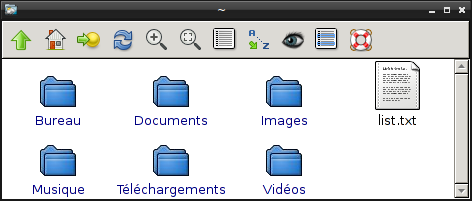
\includegraphics[width=0.7\textwidth]{rox1}
  \caption{\footnotesize{Le répertoire personnel /home/martin.albert}}
  \label{fig:rox1}
\end{figure}
Sous Unix (et donc sous GNU/Linux aussi), tous les fichiers sont regroupés dans une arborescence unique ; le sommet de cette arborescence est un répertoire appelé racine\footnote{Oui, en informatique les arbres poussent à l'envers, les racines sont en haut et les feuilles en bas.} et noté /.\par
Cette racine possède plusieurs sous-répertoires (voir figure \ref{fig:rox2}) dont les principaux sont :
\begin{description}
\item[home :] qui contient les données de tous les utilisateurs, il y a un sous-répertoire par utilisateur ;
\item[bin :] une partie des programmes installés ;
\item[mnt et media :] c'est ici qu'on retrouve les données stockées sur les autres disques durs, les clés USB, les lecteurs de médias \dots
\end{description}
\begin{figure}[ht]
  \centering
  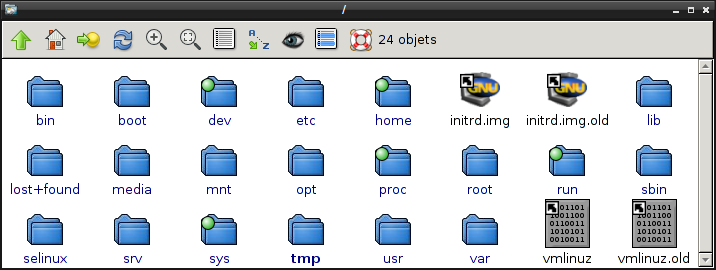
\includegraphics[width=0.7\textwidth]{rox2}
  \caption{\footnotesize{Le répertoire racine}}
  \label{fig:rox2}
\end{figure}
Sous Microsoft Windows, il y a une arborescence par périphérique de stockage de masse, chacun d'entre eux étant représenté par une lettre majuscule puis :\textbackslash. Par exemple C:\textbackslash pour le disque dur principal, D:\textbackslash pour le lecteur de DVD ou Blu Ray \dots. \par
Vous devez savoir vous repérer dans une arborescence notamment savoir retrouver votre répertoire personnel. Vous devez aussi savoir vous déplacer dans cette arborescence au moyen d'un shell graphique ou texte. Dans une shell Unix la commande pour changer de répertoire est \emph{cd} (pour change directory), pour remonter dans le répertoire parent il suffit d'utiliser \emph{cd ..}. le symbole \emph{..} représente le répertoire parent du répertoire courant qui lui est représenté par \emph{.} comme vous pouvez le voir sur la figure \ref{fig:shelltexte}.\par
De plus vous allez être rapidement amené à organiser votre propres données et un peu de méthode permettra de mieux vous repérer. N'hésitez pas à utiliser des sous répertoires pour classer les fichiers faisant partie d'une catégorie particulière. Par exemple dans votre répertoire travail, vous créez un sous-répertoire python ou vous pouvez stocker tous vos scripts python.\par
Un fichier n'est qu'une séquence finie d'octets, sans signification a priori : c'est le programme qui lira cette séquence d'octets qui décidera de la façon de l'utiliser. Sous Unix un répertoire est aussi un fichier qui ne contient qu'une liste de couples ($n$, $i$) où $n$ est le nom du fichier et $i$ son \emph{inode} qui permet d'avoir accès aux méta-données du fichier qui sont stockées dans la table des inodes :
\begin{itemize}
\item la date de création, de dernière modification et de dernière lecture ;
\item la taille du fichier ;
\item emplacement des données sur le disque.
\end{itemize}

. Ainsi on dit souvent que sous Unix tout est fichier (même les périphériques d'entrée sortie sont représentés par des fichiers).
\subsection{Droits d'accès}
En parcourant l'arborescence, Albert Martin remarque que dans le répertoire /home il y a trois autres répertoires : martin.albert qui est son répertoire personnel puis reine.benedicte et cancanier.jean qui sont les répertoires personnels de deux de ses camarades. Il décide de les visiter mais lorsqu'il clique sur le répertoire cancanier.jean il obtient le message d'erreur présenté sur la figure \ref{fig:erreur1}.
\begin{figure}[ht]
  \centering
  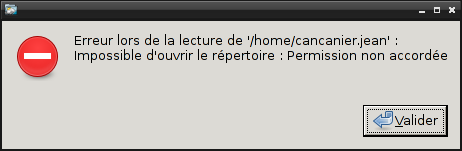
\includegraphics[width=0.6\textwidth]{erreur1}
  \caption{\footnotesize{Refus d'accès à /home/cancanier.jean}}
  \label{fig:erreur1}
\end{figure}
En revanche, il parvient à lire le répertoire /home/reine.benedicte. Celui-ci contient un fichier Lisez-moi.txt qu'Albert Martin parvient à ouvrir. Avec un éditeur de texte, il réussit à éditer le fichier mais lorsqu’il essaie de l’enregistrer, il obtient un message d’erreur présenté sur la figure \ref{fig:erreur2}. Le problème persiste s'il essaie d'enregistrer le fichier sous un autre nom.\par
\begin{wrapfigure}{r}{0.4\textwidth}
  \centering
  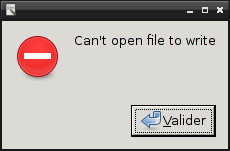
\includegraphics[width=0.325\textwidth]{erreur2}
  \caption{\footnotesize{Échec de l'enregistrement d'un fichier protégé en écriture}}
  \label{fig:erreur2}
\end{wrapfigure}
Chaque entrée de la table des inodes comporte, en plus des méta-données déjà mentionnées, les droits d'accès accordés aux utilisateurs du système. Ces droits ou permissions précisent qui à quels droits sur le fichier ou le répertoire concerné. Ces permissions sont accessibles avec la commande \emph{ls -l} dans un shell texte ou alors avec un clic droit sur le fichier ou répertoire concerné dans un shell graphique.\par
Ainsi, si on regarde les permissions de /home/cancanier.jean, les droits sont les suivants (voir figure \ref{fig:droit1}) :
\begin{figure}[ht]
  \centering
 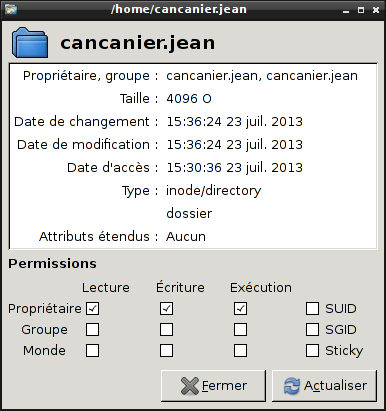
\includegraphics[width=0.6\textwidth]{droit1}
  \caption{\footnotesize{Les droits du répertoire /home/cancanier.jean}}
  \label{fig:droit1}  
\end{figure}
\begin{itemize}
\item le propriétaire du fichier est l'utilisateur cancanier.jean ;
\item le groupe auquel appartient le fichier est aussi cancanier.jean ;
\item le propriétaire du fichier peut accéder en lecture et en écriture au fichier ;
\item les autres utilisateurs n'ont aucun droit sur le fichier. 
\end{itemize}
Ainsi Albert Martin n'a pas les droits pour lire le contenu du répertoire /home/cancnier.jean d'où le premier message d'erreur (figure \ref{fig:erreur1}). \par
Dans le cas présenté figure \ref{fig:erreur2} Albert Martin essaie d'écrire sur un fichier sur lequel il n'a pas le droit d'écriture, comme on peut le constater figure \ref{fig:droit2}.
\begin{figure}[ht]
  \centering
  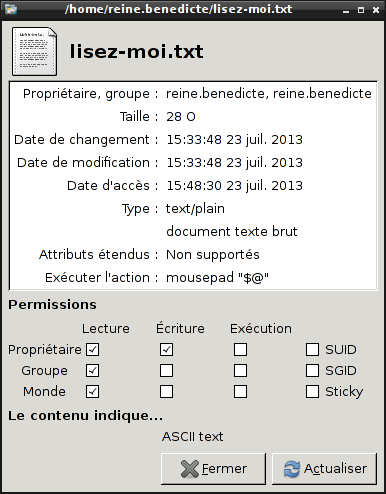
\includegraphics[width=0.6\textwidth]{droit2}
  \caption{\footnotesize{Les droits du fichier Lisez-moi.txt}}
  \label{fig:droit2}
\end{figure}
S'il essaye d'enregistrer le fichier sous un autre nom, il essayer d'écrire dans le répertoire /home/reine.benedicte sur lequel il n'a pas le droit en écriture, d'où le message d'erreur identique.\par
Tenter d'accéder aux données d'autrui peut être considéré comme une atteinte à la vie privée. De la même manière qu'on entre pas dans une maison inconnue même si la porte n'est pas verrouillée on ne cherche pas à accéder aux données d'une personne même s'il elle n'a pas bien définit les droits d'accès. Il convient d'en demander d'abord l'autorisation.\par
Passer outre une interdiction voire même se passer d'autorisation est pénalement répréhensible (art. 323-1 et suivants du code pénal). Et les peines encourues sont particulièrement lourdes : par exemple le simple fait d'accéder à un système informatique ou à des données en sachant qu'on n'en n'a pas l'autorisation, sans intention de commettre de dégâts, sans même commettre le moindre dégât involontaire, même si aucune protection n'est en place, est passible de 2 ans d'emprisonnement et 30 000 euros d'amende. 
%%% Local Variables: 
%%% mode: latex
%%% TeX-master: "cours-ipt"
%%% End: 











